\begin{section}{Tabu-Search}
	\begin{subsection}{Explicación}
		Finalmente implementamos una metaheuristica, es decir, una heurística que guía otra heurística, en este caso la búsqueda local del ejercicio anterior.

		El \texttt{Tabu-Search} permite evitar que la heurística de búsqueda local se estanque en óptimos locales cuando en realidad fuera de la vecindad existía una solución óptima global (mejor que la local).
		Para lograrlo, permite al algoritmo perseguir una solución peor que la mejor obtenida mediante búsqueda local, por una cantidad máxima de iteraciones.
		Pasada esta cantidad, con-\\sideramos que el algoritmo ya buscó lo suficiente y la mejor solución encontrada hasta el momento debe ser la óptima.

		Para no revisar las vecindades que se revisaron anteriormente (que son muy cercanas a la vecindad actual),
		cada vez que decidimos movernos a otra vecindad porque tenemos un nuevo aspirante a óptimo (más allá de que sea peor que la mejor solución que encontramos hasta el momento, pero lo llamamos así por su similitud con el mismo en la búsqueda local)
		prohibimos revertir el cambio que hicimos para llegar del aspirante anterior al nuevo, o sea, prohibimos volver a agregar el vértice que sacamos.
		
		Cada vez que logramos mejorar, es decir, encontramos una clique de tamaño mayor a la máxima clique vista hasta el momento actualizamos la solución.
		Repetimos este procedimiento hasta agotar la máxima cantidad de iteraciones permitidas sin mejorar. Una vez que ocurre esto, el algoritmo termina, siendo la solución final la solución actual, es decir, la clique de mayor tamaño que logro encontrar.(Figura \ref{fig:seguimiento_busqueda_tabu})

			% --- Figura seguimiento algoritmo constructivo ---
			\begin{figure}[H]
				\centering
		    	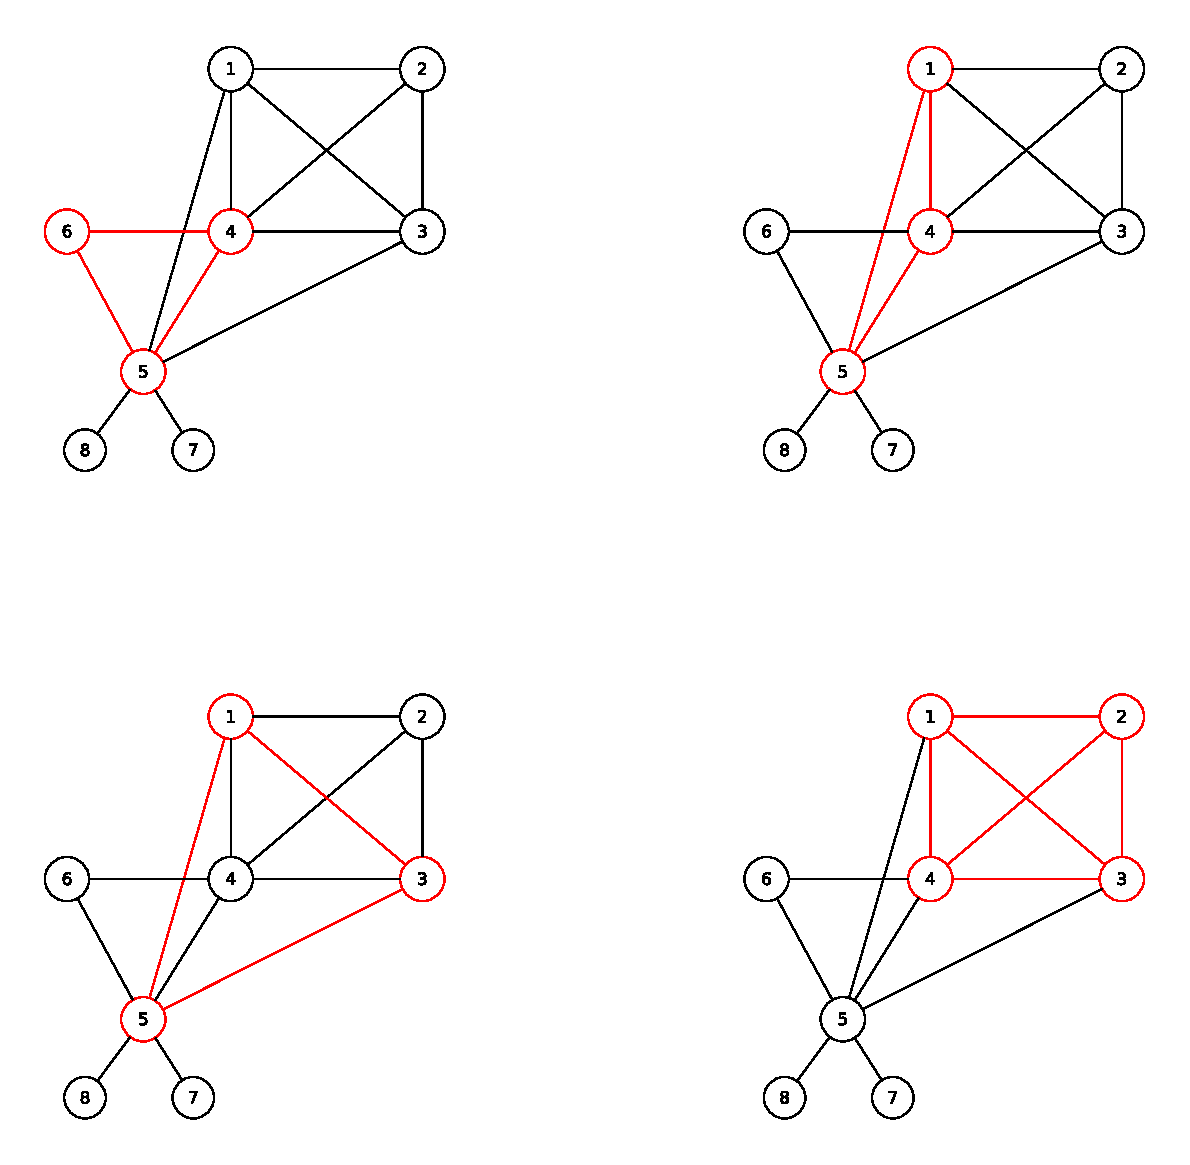
\includegraphics[scale=0.5]{tabu_search/seguimiento.eps}
			    \caption{Ejemplo de la heurística de búsqueda tabú}
			    \label{fig:seguimiento_busqueda_tabu}
			\end{figure}

		CARLANCHA LOQUIÑA TENES Q AGREGARLE MIL MIL MIL MIL NODOS AL SEIS XQ SINO ES REQUETE VERSO ESTO

		La heurística de búsqueda local nos da la clique formada por $<4,5,6>$ SARARARARARARASASASASA

		\begin{comment}
		Esto lo implementamos mediante un arreglo de vértices (los índices representan los vértices), donde para cada uno guardamos la cantidad de iteraciones que falta para que deje de ser tabú (el algoritmo lleva la cuenta de las iteraciones).
		Luego, cuando revisamos las vecindades de un aspirante, evitamos aquellas donde la modificación implica agregar un vértice tabú.

		Los parámetros que indican cuanto tiempo una variable queda tabú y cuantas veces se puede iterar sin encontrar un nuevo óptimo antes de cortar el algoritmo, los buscamos empíricamente viendo los resultados obtenidos con distintos parámetros, y son bla y bla respectivamente.
		CAMBIAR LOS PARAMETROS!!!
		\end{comment}
	\end{subsection}
	\begin{subsection}{Detalles de la implementación}
		Almacenamos las relaciones entre los vértices en una matriz de $n \times n$, donde $n$ es la cantidad de vértices. Cada posición $(i,j)$ de la matriz contiene un $uno$ si existe la arista $(i,j)$ y un $cero$ en caso contrario. De esta forma se le asigna un número a cada vértice.\VSP

		A continuación, se muestra el pseudocódigo de la heurística de búsqueda tabú.\\

		Sea $n$ la cantidad de vértices del grafo.

		\begin{pseudo}
			\func{busqueda\_tabu}{solucion,tamanyo,matriz\_adyacencia}
			\tab $\IF tamanyo==1 \OR tamanyo==n$\\
			\tab \tab $\RET tamanyo$\\
			\tab $grados[n] \leftarrow ordenar\_grados(matriz\_adyacencia)$\\
			\tab $\WHILE mejore$\\
			\tab \tab $\FOR c \TO tamanyo$\\
			\tab \tab \tab $inicializar\_estructuras$\\
			\tab \tab \tab $rotar\_clique$\\
			\tab \tab \tab $\WHILE puedo\;seguir$\\
			\tab \tab \tab \tab $sacar\_de\_clique$\\
			\tab \tab \tab \tab $poner\_tabu$\\
			\tab \tab \tab \tab $formar\_completo(actual,matriz\_adyacencia)$\\
			\tab \tab \tab \tab $\IF tam\_actual>tamanyo$\\
			\tab \tab \tab \tab \tab $agrandar\_clique(actual,lista\_tabu)$
			\tab \tab \tab \tab \tab $actualizar\_solucion$
			\tab \tab \tab \tab \tab $c \leftarrow tamanyo$\\
			\tab \tab \tab \tab $\ELSE$\\
			\tab \tab \tab \tab \tab $restar\_tabu$\\
			\tab \RET $tamanyo$\\
		\end{pseudo}

		En la implementación mantenemos la solución actual tanto en una lista de vértices. La lista inicia ordenada de mayor a menor según los grados, esto lo hacemos para empezar a sacar desde el de menor grado ya que consideramos que es el que tiene más probabilidades de estar condicionando la clique. Además, tenemos un arreglo de tipo bool de tamaño $n$ donde el índice representa a los vértices y esta seteado en $verdadero$ si y sólo si el vértice pertenece a la clique actual. Mantenemos ambas estructuras porque usamos la lista para determinar el orden en que se eliminan (rotarla tiene costo constante) y el arreglo para verificar la pertenencia de un vértice a la clique (ya que esta operación en esta estructura de datos tiene costo constante).
		Por otro lado, mantenemos un arreglo de vértices (los índices representan los vértices), donde para cada uno guardamos la cantidad de iteraciones que falta para que deje de ser tabú una vez que son eliminados de la clique actual (el algoritmo lleva la cuenta de las iteraciones). Esto lo hacemos para no revertir los cambios recientemente hechos y cuando revisamos las vecindades de un aspirante, evitamos aquellas donde la modificación implica agregar un vértice tabú.

		La primer cláusula \texttt{if} verifica si la solución de búsqueda local encontró la clique tanto completa como la de un elemento. En ambos casos no tiene sentido aplicar el tabú search ya que, si encontró el completo, esta solución no podrá ser mejorada, al contener todos los vértices. Si sólo encontró un vértice, implica que el de grado mayor en el grafo es de grado cero, por lo tanto, todos sus vértices son de grado cero.

		El valor de verdad de la guarda del \texttt{while} $puedo\_seguir$ viene dado por la conjunción entre $tam\_actual \neq 1$, $\neg mejore$ e $iteracion<n$.
		Pedimos que el tamaño de la clique actual sea distinto de $uno$ ya que nos interesa movernos a soluciones vecinas. Si el tamaño es $uno$ en esa iteración saca el último vértice de la clique por lo que se pierde referencia a la misma moviéndose inmediatamente al primer vértice segun la numeración que no esté tabú.
		Por otro lado, el \texttt{while} itera mientras no logre mejorar para forzar la salida del ciclo cuando encuentre una clique de mayor tamaño que la actual y así empezar a sacar vértices desde la primer rotación (ya que también se fuerza la salida del \texttt{for}).
		La última condición es para asegurar la salida del ciclo, ya que podría no mejorar nunca y ciclar entre diferentes cliques. Además, esto determina la cantidad de iteraciones que le permitimos buscar sin lograr mejorar, es un parámetro que ajustamos de la siguiente manera AJUSTEMOSLO ALGUN DIAAAAAA!!!!!ukuyfuyjtjft5umj76fu7666m,6b,ib7,ki7k,i87fk7k,KUFMKUTJYTDMHYTMJUY6FMJUYMKY

		\begin{itemize}			
			\item \texttt{rotar\_clique: } Dado que fijar la pertenencia de un vértice a la clique condiciona el resultado final, el orden en que se eliminen los vértices puede hacer la diferencia entre un buen resultado y uno malo, a pesar de encontrar un buen criterio para hacerlo. Por este motivo, decidimos empezar eliminando de menor a mayor grado, y en cada iteración rotar la lista para sacar los vértices en otro orden.
			
			\item \texttt{sacar\_de\_clique: }Esta función saca de la lista el último elemento (el de menor grado entre los vértices con una misma 'antiguedad' en la clique) y setea en $falso$ la posición correspondiente en el arreglo (dejando tabú la operación inversa (agregarlo a la clique) tantas iteraciones como el tamaño de la clique con la que empieza a sacar), es decir, excluye el vértice de la solución actual. Además, decrementa la variable que indica el tamaño de la clique.

			LA CANTIDAD DE ITERACIONES QUE QUEDA TABU ES UN PARAMETRO ARREGLARLO
			
			\item \texttt{formar\_completo: } Esta función se encarga de buscar entre los vértices que actualmente no pertenecen a la clique e intenta agregarlos (agrega todo vértice que forma un completo con los ya pertenecientes), con el objeto de conseguir una de mayor tamaño. Para saber si agregarlo determina una solución al problema debemos verificar que forme un completo con los vértices ya incluídos. Para esto recorremos todos los vértices del grafo y para cada uno que pertenezca a la solución parcial chequeamos que sea adyacente al que pretendemos agregar. Si esto ocurre podemos agregarlo y agrandar la clique. Elegimos el vértice a agregar de mayor a menor grado.
			
			\texttt{Observaciones: }
			\begin{itemize}
				\item Al agregar condicionamos la clique resultante al igual que pasa al sacar sin hacer rotaciones (depende del orden en que lo hagamos la calidad de la solución). Es decir, encontrar una mejor solución depende del orden en que agreguemos los vértices, podriamos también hacer rotaciones para agregar pero esto aumentaría en $n$ la complejidad. Buscando un equilibrio entre eficiencia y calidad de la solución, decidimos que hacer ambas rotaciones (agregar, sacar) tenia una complejidad mayor a la que pretendemos aceptar, no hacer ninguno implica perdernos de encontrar mejores soluciones y obtener así soluciones muy precarias. Entonces elegimos arbitrariamente hacer las rotaciones sólo para sacar.

				\item Si el algoritmo vuelve a la solución inicial y todavía le restan iteraciones del \texttt{while} anidado, queremos evitar que repita exactamente el mismo procedimiento pasando nuevamente por soluciones ya visitadas por lo que forzamos la salida y aplicamos una rotación a dicha solución para explorar nuevas posibilidades.
			\end{itemize}

			\item \texttt{agrandar\_clique: } Esta función itera los vértices que están en la lista tabú e intenta agregarlos a la clique actual. Esto es porque como ya conseguí una solución mejor lograr agregar algún vértice que esta tabú contribuye aún más a la solución.

			\item \texttt{restar\_tabu: } Para cada vértice tal que tiene tabú mayor a $cero$ decrementa la cantidad de iteraciones que va a permanecer tabú. Si al decrementarlo deja de ser tabú lo elimina de $lista\_tabu$.

			Tanto en $formar\_completo$ como en $agrandar\_clique$ los vértices que agregamos a la lista de la clique actual los ponemos al principio de la misma, es una forma de poner tabú al menos tantas iteraciones como vértices había en la clique previo a agregarlos la operación inversa, sacarlos (ya que se saca siempre el último de la lista).
		\end{itemize}
	\end{subsection}

	\begin{subsection}{Desventajas}
		La numeración de los nodos toma un papel crucial a la hora de obtener una solución, es así que en casos patológicos puede pasar que:

		El algoritmo visite soluciones anteriormente exploradas ya que como se mueve constantemente de solución, puede eventualmente volver a la solución inicial (ejemplo: la búsqueda local nos da un clique de dos vértices que se encuentran en un ciclo, y este ciclo está unido a un completo de tres o más vértices). Si los vértices del completo tienen mayor numeración a los del ciclo, el algoritmo ciclaría tomando en cada iteración (mientras no se cumpla la restricción de iteraciones pasadas como parámetros) como solución dos de los vértices pertenecientes al ciclo, sin ver el completo.

		Para evitar pasar varias veces por las mismas soluciones, por cada iteración del \texttt{while} anidado se verifica si vuelve a la solución inicial, de ser así, se fuerza la salida y se procede a la siguiente rotación de la clique.
		A pesar de solucionar este problema para casos particulares como el que mencionamos (donde se parte de una solución y a través eliminar y agregar vértices se llega nuevamente a la solución inical), pueden existir casos donde se repitan soluciones desde distintas rotaciones de la clique inicial. Estos casos no son advertidos por el algoritmo.
	\end{subsection}

	\begin{subsection}{Complejidad temporal}
			En un pricipio el algoritmo inicializa el arreglo de los $grados$ y lo ordena, lo que tiene un costo de $n^2$ ya que se utiliza el algoritmo de ordenamiento $QuickSort$. Luego, obtiene la solución inicial mediante la heurística de busqueda local que como ya vimos tiene un costo de $n^4$.

			La función $rotar\_clique$, $sacar\_de\_clique$ y $poner\_tabu$ tienen costo\\ constante ya que constan sólo de indexaciones, asignaciones y operaciones elementales sobre listas.

			La función $formar\_completo$ itera por todos los vértices y para cada uno de estos verifica si es factible agregarlo a la clique, lo cual tiene un costo de $n^2$ ya que dicha verificación consiste en recorrer todos los vertices del grafo y ver que el vértice que se pretende agregar es adyacente a cada uno de estos. Además, se concatena la lista de los vértices agregados con la lista de la clique actual lo que tiene un costo constante.

			La función $agrandar\_clique$ tiene costo $n^2$ ya que no es más que una llamada a la función $formar\_completo$ con todos los vértices permitidos, es decir, previo a la llamada se resetea el arreglo $tabu$.

			 La cantidad de iteraciones del primer ciclo \texttt{while} se puede acotar por $n$ (seria un caso hipotetico en el que la mejora sea sólo de un vértice, es decir, se inicie con la clique trivial (tamaño $uno$) y en cada iteración de este ciclo se logre incrementar en uno el tamaño de la clique). En cada una de estas iteraciones hay un ciclo \texttt{for} que se ejecuta a lo sumo tantas veces como el tamaño de la clique, también puede ser acotado por $n$, dentro de este ciclo se resetean las estructuras (la lista y los arreglos) lo que tiene un costo lineal. Además, hay un ciclo \texttt{while} (dentro del for) que se ejecuta a los sumo $n$ veces y en cada una de las iteraciones hay una llamada a la función $sacar\_de\_clique$ con costo constante y $formar\_completo$ con costo $n^2$, en caso de lograr mejorar hay una llamada a la función $agrandar\_clique$ con costo $n^2$, en caso contrario, hay una llamada a la función $restar\_tabu$ de costo lineal (recorre todos los vértices decrementando la cantidad de iteraciones que permaneceran tabú). Entonces la complejidad del \texttt{while} anidado es:  \Ode{n*(\Ode{sacar\_de\_clique} + \Ode{formar\_completo} + \Ode{agrandar\_clique} + \Ode{restar\_tabu})} = \Ode{n*(1+n^2+n^2+n)} = \Ode{n^3}.

			 Finalmente, se deduce que la complejidad final del algoritmo es $n^5$ ya que acotamos tanto la cantidad de iteraciones del cliclo \texttt{while} como del \texttt{for} por $n$, entonces tenemos \Ode{n*n*\Ode{while\_anidado}}=\Ode{n^5}.\Pa
			 
			 \texttt{Observación: } En la función $formar\_completo$ para ver si es factible agregar un vértice a la clique en vez de recorrer todos los vértices del grafo como hacemos, se podria sólo recorrer los vértices pertenecientes a la clique ya que están en una lista, pero la complejidad sería la misma y deberiamos ir agregando a la lista a medida que se decide agregar un vértice (para considerarlo en las proximas verificaciones) y esto no nos permite hacerlo en el orden deseado (ya que queremos agregar al principio de la lista de la clique actual de menor a mayor grado y los recorremos de mayor a menor grado). Como ya mencionamos esto no mejoraria la complejidad asintotica y aumentaria la complejidad de comprensión del código.
	\end{subsection}

\end{section}
